\subsection{Persistenslag}
\label{sub:persistenslag}

Persistenslagsmodulet har til opgave at manipulere og læse data fra en vilkårlig datastruktur.

\subsubsection{Funktionalitet}
\label{ssub:persistenslag_funktionalitet}

En datastruktur kunne eksempelvis være en database eller en anden fil på harddisken. Modulet tilbyder basale CRUD (create, read, update og delete) operationer, hvorfra alle tænkelige persistenslagsoperationer kan opbygges af.

Et eksempel på brugen af persistenslagsmodulet, kunne være loginmodulet. Loginmodulet skal verificere om et indtastet brugernavn matcher et indtastet kodeord. Til dette kan loginmodulet tilgå databasen igennem persistenslagets read operation, og herfra arbejde videre på den fundne data.

\subsubsection{Implementation}
\label{ssub:persistenslag_implementation}
\begin{figure}
  \centering
  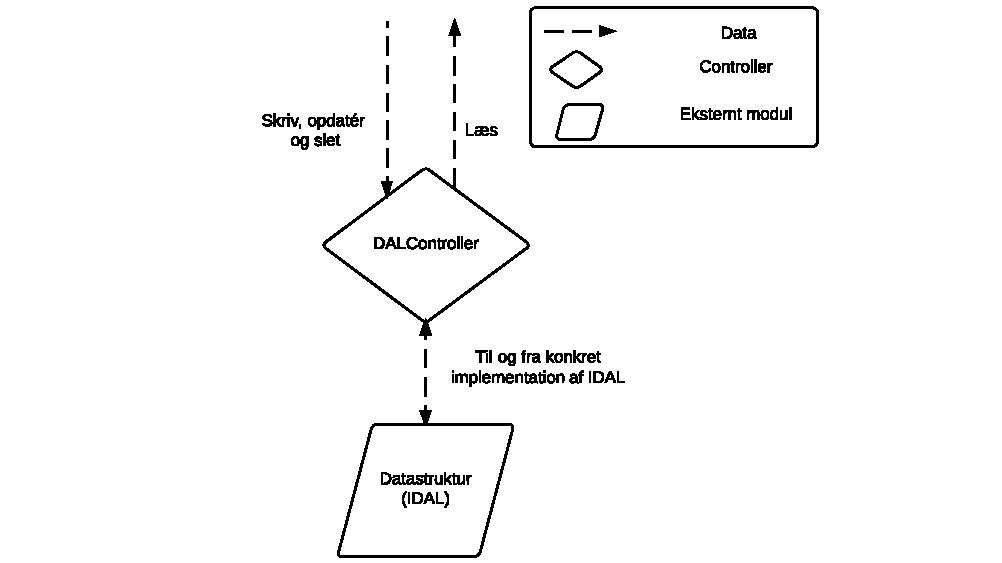
\includegraphics[width=\textwidth]{persistenslag-diagram.pdf}
  \caption{dette er tekst for tekst skyld }
  \label{fig:permod}
\end{figure}
\frnote{lidt tekst til billedet}

Persistenslagsmodulet er opbygget således at selve datastrukturen der manipuleres og læses fra, kan skiftes ud. Herved indkapsles tilgangen til datastrukturen på en sådan måde, at et program kan gå fra at benytte en xml fil som data lager, til at benytte en database uden at ødelægge anden eksisterende kode.

Som man kan se på \cref{fig:permod} består persistenslagsmodulet af en enklet klasse DALController. Denne klasse er kun bevidst om en konkret implementation af tilgangen til en datastruktur. Dette sker via interfacet IDAL. Når et andet modul ønsker at lave en læse operation på persistenslag modulet, videredelegeres denne operation til den underliggende implementation af tilgangen til en datastruktur.